\documentclass{report}
\usepackage{polyglossia}
\usepackage{fixlatvian}
\usepackage{graphicx}
\usepackage{circuitikz}
\usepackage{tabularx}
\usepackage{verbatim}
\usepackage{float}
\usepackage{pgfplots}
\graphicspath{{atteli/}}
\title{Laboratorijas darba atskaite}
\author{Viktorija Trofimova}

\begin{document}
\maketitle
%=============================
\chapter{Teorētiskā daļa}
\section{Ķēdes aprēķins}

Apēķiniet spriegumus uz rezistoriem 1. attēlā dotajā shēmā. Sprieguma avota V1 spriegu-
ma vērtību U (Voltos) izvēlieties daļskaitli, kas būtu Jūsu apliecības pēdējie trīs cipari dalīti ar
10. Piemēram. ‘ 101REB123 ’ nozīmē V1 = 12.3 (Volti), R1 ir apliecības pēdējo 3 ciparu otrais
numurs+1, R2 ir apliecības numura pēdējais cipars +1. Piemēram, ja Jūsu apliecības numurs
ir ‘ 101REB123 ’ tad ‘ R1=3 ’, ‘ R2=4 ’. Nofotografējiet aprēķinu vai saglabājiet lapiņu. Aprēķina gaita
būs nepieciešama darbā ‘ P02 ’. Turklāt, aprēķins būs jāpievieno atskaitei, ko veiksiet semestra
beigās.


\begin{table}[h]
\centering
\begin{tabular}[h]{|c|c|}
\hline
$R1$ & 9 $\Omega$\\
\hline
$R2$ & 9 $\Omega$\\
\hline
$V1$ & 18.8 V\\
\hline
$U_{R_1}$ & 9.4 V\\
\hline
$U_{R_2}$ & 9.4 V\\
\hline
\end{tabular}
\caption{}
\label{table:ta}
\end{table}



\begin{figure}[t]
\centering
\begin{circuitikz}
\draw
(0,0) to[battery=$V$1] (0,4)
to[european resistor, l_=$R_1$] (4,4)
to[european resistor, l_=$R_2$] (4,0) -- (0,0)
;
\end{circuitikz}
\caption{}
\label{fig:sh}
\end{figure}

\begin{figure}[!b]
\centering
\begin{tikzpicture}
\begin{axis}[
    title={$U_{R_{2}}=f(R_2)$},
    xlabel={$R_2$ [$\Omega$]},
    ylabel={$U_{R_{2}}$ [V]},
    xmin=5, xmax=50,
    ymin=5, ymax=15,
    xtick={0,10,20,30,40,50},
    ytick={0,5,10,15},
    ymajorgrids=true,
    xmajorgrids=true,
    grid style=dashed,
]
\addplot[color=blue,]
    coordinates {
    (5,6.71)(10,9.47)(15,11)(20,11.9)(25,12.6)(30,13.1)(35,13.4)(40,13.7)(45,13.9)(50,14.1)
    };
\end{axis}
\end{tikzpicture}
\caption{}
\label{fig:gr}
\end{figure}
%=============================
\chapter{Praktiskā daļa}
\section{Darbs ar GEDA programmām}
\subsection{Darbs ar gschem}
\begin{figure}[h]
    \centering
    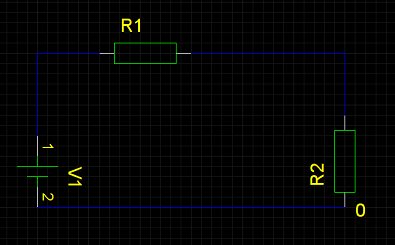
\includegraphics{gschem01.png}
    \caption{}
    \label{fig:sh2}
\end{figure}

\newpage
\subsection{Darbs ar gnetlist}
\verbatiminput{atteli/01.net}

\subsection{Darbs ar ngspice}
Skatīt attēlus \ref{fig:2.1} un \ref{fig:2.2} 
\begin{figure}[!h]
    \centering
    \includegraphics[width=10cm]{011.ps}
    \caption{Spriegums 1.vadā}
    \label{fig:2.1}
    \end{figure}
 \begin{figure}[t]
 \centering
    \includegraphics[width=10cm]{012.ps}
    \caption{Spriegums 2.vadā}
    \label{fig:2.2}
\end{figure}
\newpage

\section{Darbs ar QUCS programmām}
\begin{figure}[!h]
    \centering
    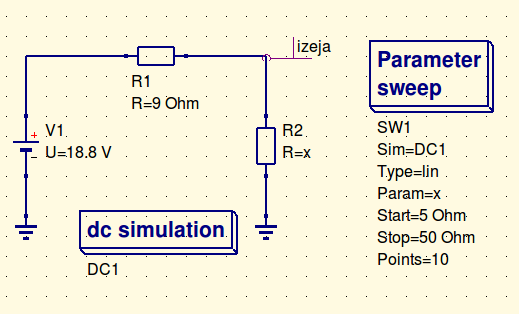
\includegraphics[width=\textwidth, height=\textheight, keepaspectratio]{qucs02sch.png}
    \caption{QUCS shēma}
    \label{fig:2.3}
    \end{figure}
 
\begin{figure}[t] 
\centering
    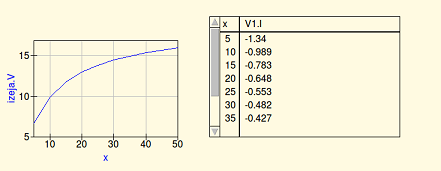
\includegraphics[width=\textwidth, height=220 pt, keepaspectratio]{qucskopa.png}
    \caption{Sweep simulācijas tabula, līdzstrāvas simulācijas grafiks}
    \label{fig:2.4}
\end{figure}

\newpage

\label{s_nobeigums}

\begin{thebibliography}{9}
\bibitem{1} 
\textit{Bibliography management.} [Skatīts 2018. gada 05. jūnijā].
Pieejams: https://www.sharelatex.com/learn/Bibliography\_{}management\_{}in\_{}LaTeX

\bibitem{2} 
\textit{Tables.} [Skatīts 2018. gada 05. jūnijā].
Pieejams: https://www.sharelatex.com/learn/Tables
 
\end{thebibliography}

\end{document}
